\documentclass[a4paper,12pt]{article}
\usepackage{polski}
\usepackage[utf8]{inputenc}
\usepackage[left = 3cm, right = 3cm, top = 2cm, bottom = 2cm]{geometry}
\usepackage{enumerate}
\usepackage{amssymb}		% pakiet do symboli
\usepackage{mathtools}		% pakiet do matmy (rozszerza amsmath)
\usepackage{enumitem}		% punktowanie (a), (b), ...
\usepackage{nopageno}		% brak numerow stron
\usepackage{graphicx}		% wstawianie obrazkow
\usepackage{float}			% wstawianie obrazkow w dowolnym miejscu
\usepackage{caption}
\usepackage{esdiff}         % pochodne \diff{}{}
\usepackage{listings}
\usepackage{xcolor}
\usepackage{adjustbox}
\usepackage{tkz-graph}
\usepackage{pgfplots, pgfplotstable}
\usepackage{esint}
%\usepackage[none]{hyphenat} % usunięcie łamania wyrazów na końcu linii

% nowe komendy dla wygodniejszego pisania :)
\newcommand{\comment}[1]{}                              % zjedz wszystko w środku
\newcommand{\floor}[1]{\left\lfloor #1 \right\rfloor}	% podłoga
\newcommand{\ceil}[1]{\left\lceil #1 \right\rceil}		% sufit
\newcommand{\fractional}[1]{\left\{ #1 \right\}}		% część ułamkowa {x}
\newcommand{\abs}[1]{\left| #1 \right|}					% wartosc bezwzgledna / moc
\newcommand{\set}[1]{\left \{ #1 \right \}}				% zbiór elementów {a,b,c}
\newcommand{\pair}[1]{\left( #1 \right)}				% para elementów (a,b)
\newcommand{\Mod}[1]{\ \mathrm{mod\ #1}}				% lekko zmodyfikowane modulo
\newcommand{\comp}[1]{\overline{ #1 }} 					% dopełnienie zbioru 
\newcommand{\annihilator}{\mathbf{E}}					% operator E
\newcommand{\seqAnnihilator}[1]{\annihilator \left\langle #1 \right\rangle} % E(a_n)
\newcommand{\sequence}[1]{\left\langle #1 \right\rangle} % <a_n>
\newcommand{\subst}[1]{}
\DeclareMathOperator{\lcm}{lcm}							% obsługa lcm w mathmode

% styl do kodu
\lstdefinestyle{code}{%
basicstyle=\ttfamily\small,
commentstyle=\color{green!60!black},
keywordstyle=\color{magenta},
stringstyle=\color{blue!50!red},
showstringspaces=false,
numbers=left,
numberstyle=\footnotesize\color{gray},
numbersep=10pt,
tabsize=4,
rulecolor=\color{red},
breaklines=true
}

\newcommand{\code}[1]{\lstinline[style=code]{#1}} % kod inline

% tutaj coś do rysowania dystrybuanty
\makeatletter
\long\def\ifnodedefined#1#2#3{%
    \@ifundefined{pgf@sh@ns@#1}{#3}{#2}%
}

\pgfplotsset{
    discontinuous/.style={
    scatter,
    scatter/@pre marker code/.code={
        \ifnodedefined{marker}{
            \pgfpointdiff{\pgfpointanchor{marker}{center}}%
             {\pgfpoint{0}{0}}%
             \ifdim\pgf@y>0pt
                \tikzset{options/.style={mark=*, fill=white}}
                \draw [densely dashed] (marker-|0,0) -- (0,0);
                \draw plot [mark=*] coordinates {(marker-|0,0)};
             \else
                \tikzset{options/.style={mark=none}}
             \fi
        }{
            \tikzset{options/.style={mark=none}}        
        }
        \coordinate (marker) at (0,0);
        \begin{scope}[options]
    },
    scatter/@post marker code/.code={\end{scope}}
    }
}
\makeatother

% a to do lepszych granic w podwojnych i wielokrotnych calkach
\makeatletter
%% make esint definition in line with amsmath
\@for\next:={int,iint,iiint,iiiint,dotsint,oint,oiint,sqint,sqiint,
  ointctrclockwise,ointclockwise,varointclockwise,varointctrclockwise,
  fint,varoiint,landupint,landdownint}\do{%
    \expandafter\edef\csname\next\endcsname{%
      \noexpand\DOTSI
      \expandafter\noexpand\csname\next op\endcsname
      \noexpand\ilimits@
    }%
  }
\makeatother

\begin{document}
\noindent \textbf{RPiS, Lista 1 - Tomasz Woszczyński}\newline

\noindent \newline \textbf{Zadanie 1} \newline
Niech $\Sigma$ będzie $\sigma$-ciałem zbiorów.
\begin{enumerate}[label=(\alph*)]
    \item Sprawdzić, że $\emptyset \in \Sigma$.
    \item Załóżmy, że $A_k \in \Sigma$, dla $k = 1, 2, 3, \ldots$. Wykazać, że
            $\bigcap\limits_{k \in \mathbb{N}} A_k \in \Sigma$.
\end{enumerate}

\noindent \textbf{Podpunkt (a):} \\
Zgodnie z definicją rodziny zdarzeń, $\Omega \in \mathcal{F}$ oraz jeśli
$A \in \mathcal{F}$, to dopełnienie zbioru $A$ również należy do $\mathcal{F}$.
Skoro tak, to dopełnieniem zbioru $A = \Omega$ jest $A^\complement = 
\Omega \setminus \Omega = \emptyset$.\\

\noindent \textbf{Podpunkt (b):} \\
Wiemy, że dla $A_k \in \Sigma$ zachodzi $A_k^\complement = (\Omega \setminus A_k)
\in \Sigma$, czyli $\bigcup\limits_{k \in \mathbb{N}} (\Omega \setminus A_k) =
\bigcup\limits_{k \in \mathbb{N}} A_k$. Ponadto, skorzystajmy z prawa de Morgana:
\[
    \left(
        \bigcup\limits_{i \in I} A_i
    \right)^\complement 
    = \bigcap\limits_{i \in I} A_i^\complement, 
    \text{ gdzie } I \in \mathbb{N}
\]

\noindent Dzięki temu możemy wykonać następujące przekształcenia:
\[
    \bigcup\limits_{k \in \mathbb{N}} A_k =
        \bigcup\limits_{k \in \mathbb{N}} (\Omega \setminus A_k) =
        \bigcup\limits_{k \in \mathbb{N}} (\Omega \setminus A_k)^\complement =
        \bigcap\limits_{k \in \mathbb{N}} A_k, \text{ c.n.d.}
\]

\noindent \newline \textbf{Zadanie 2} \newline
Niech $\Omega = \set{a, b, c}$.
\begin{enumerate}[label=(\alph*)]
    \item Opisać $\sigma$-ciała zbiorów tej przestrzeni zdarzeń.
    \item Podać przykład funkcji $X, Y$ takich, że $X$ jest zmienną losową,
            a $Y$ nie jest zmienną losową.
\end{enumerate}

\noindent \textbf{Podpunkt (a):} \\
Wszystkimi $\sigma$-ciałami zbiorów tej przestrzeni zdarzeń są:
\begin{align*}
    \Sigma_1 &= \set{\Omega, \emptyset} \\
    \Sigma_2 &= \set{\Omega, \emptyset, \set{a}, \set{b, c}} \\
    \Sigma_3 &= \set{\Omega, \emptyset, \set{b}, \set{a, c}} \\
    \Sigma_4 &= \set{\Omega, \emptyset, \set{c}, \set{a, b}} \\
    \Sigma_5 &= \set{\Omega, \emptyset, \set{a}, \set{b}, 
        \set{c}, \set{a, b}, \set{b, c}, \set{a, c}}
\end{align*}

\noindent W pierwszym przypadku nie bierzemy żadnych "dodatkowych" zbiorów poza 
$\Omega$ i jego dopełnieniem. W kolejnych przypadkach dodajemy po kolei jednoelementowe
zbiory oraz ich dopełnienia, a więc wyczerpujemy wszystkie możliwości, gdyż dopełnienia
są wszystkimi możliwościami zbiorów dwuelementowych. W ostatnim przypadku bierzemy
jeszcze wszystkie singletony, jak i ich dopełnienia.\\

\noindent \textbf{Podpunkt (b):} \\
Weźmy sobie $\sigma$-ciało zbiorów $\Sigma_4 = \set{\Omega, \emptyset, 
\set{c}, \set{a, b}}$. Zdefiniujmy funkcję $X$ będącą zmienną losową oraz
funkcję $Y$ niebędącą zmienną losową:

\begin{minipage}{0.45\textwidth}
    \[
        X(z) = \begin{cases}
            0 & \text{ dla } z = a \text{ lub } z = b \\
            1 & \text{ dla } z = c
        \end{cases}  
    \]
\end{minipage}%%
\begin{minipage}{0.45\textwidth}
    \[
        Y(z) = \begin{cases}
            0 & \text{ dla } z = a \\
            1 & \text{ dla } z = b \text{ lub } z = c
        \end{cases}  
    \]
\end{minipage}%%

\noindent Wtedy $X(a) = 0, X(b) = 0, X(c) = 1$ oraz $X^{-1}(0) = \set{a, b}, 
X^{-1}(1) = \set{c}$. Zbiory $\set{a,b}$ i $\set{c}$ należą do $\Sigma_4$,
czyli rzeczywiście $X$ jest zmienną losową. W przypadku $Y$ mamy: $Y(a) = 0,
Y(b) = 1, Y(c) = 1$, ale $Y^{-1}(0) = \set{a}, Y^{-1}(1) = \set{b, c}$. Łatwo
zauważyć, że zbiory $\set{a}, \set{b,c} \notin \Sigma_4$, czyli nie należą do
rodziny zdarzeń, co przeczy definicji zmiennej losowej.


\noindent \newline \textbf{Zadanie 3} \newline
Niech $\Omega = \set{1, 2, 3, 4, 5}$ oraz $S = \set{1, 4}$. Wyznaczyć najmniejsze
$\sigma$-ciało zbiorów zawierające $S$. \\

\noindent $\sigma$-ciało musi zawierać $\Omega$, dla każdego elementu 
$A \in \mathcal{F}$ dopełnienie $A$ również musi należeć do $\mathcal{F}$,
oraz suma wszystkich zbiorów $A_i$ dla $i \in \mathbb{N}$ musi należeć do
$\mathcal{F}$. Biorąc pod uwagę te trzy warunki, najmniejszym $\sigma$-ciałem
zawierającym zbiór $S$ jest:
\[
    \mathcal{F} = \set{
        \Omega, 
        \underbrace{\emptyset}_{\Omega^\complement},
        \set{1, 4},
        \underbrace{\set{2, 3, 5}}_{\set{1, 4}^\complement}
    }
\]

\noindent \newline \textbf{Zadanie 4} \newline
Wyznaczyć dystrybuantę i obliczyć wartość oczekiwaną zmiennej $X$ o rozkładzie
\[
    \begin{matrix*}
        x_i &   2   &   3   &   4   &   5   \\
        p_i &   0.2 &   0.4 &   0.1 &   0.3
    \end{matrix*}
\]

\noindent Dystrybuantę możemy wyznaczyć poprzez wyznaczanie odpowiednich
wartości dla kolejnych przedziałów. Zawsze $\sum\limits_{i} p_i = 1$ (jest to
maksymalna wartość dystrybuanty, jako że jest to funkcja schodkowa i rosnąca).
Dystrybuantą dla takiego rozkładu będzie:

\begin{minipage}{0.35\textwidth}
\[
    F(x) = \begin{cases}
        0   & \text{ dla } x \in (-\infty, 2) \\
        0.2 & \text{ dla } x \in [2, 3) \\
        0.6 & \text{ dla } x \in [3, 4) \\
        0.7 & \text{ dla } x \in [4, 5) \\
        1   & \text{ dla } x \in [5, \infty) \\
    \end{cases}  
\]
\end{minipage}%%%%%%
\begin{minipage}{0.65\textwidth}
\begin{center}
    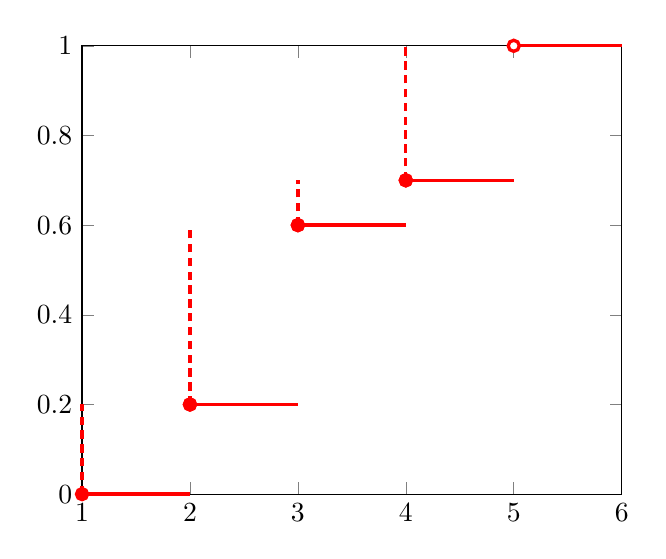
\begin{tikzpicture}
        \begin{axis}[
            clip=false,
            jump mark left,
            ymin=0,ymax=1,
            xmin=1, xmax=6,
            every axis plot/.style={very thick},
            discontinuous,
            table/create on use/cumulative distribution/.style={
                create col/expr={\pgfmathaccuma + \thisrow{f(x)}}   
            }
        ]
        \addplot [red] table [y=cumulative distribution]{
        x f(x)
        1 0
        2 0.2
        3 0.4
        4 0.1
        5 0.3
        6 0
        };
        \end{axis}
    \end{tikzpicture}
\end{center}
\end{minipage}

\noindent Wartość oczekiwaną $\mathbb{E}[X]$ zmiennej losowej obliczamy 
ze wzoru $\mathbb{E}[X] = \sum\limits_{i} x_i p_i$, czyli:
\[
    \mathbb{E}[X] = 2 \cdot 0.2 + 3 \cdot 0.4 + 4 \cdot 0.1 + 5 \cdot 0.3 =
        0.4 + 1.2 + 0.4 + 1.5 = 3.5
\]  

\newpage
\noindent \textbf{Zadanie 5} \newline
Dystrybuanta $F$ zmiennej losowej $X$ jest określona następująco:
\[
    \begin{matrix*}
        x       &   (-\infty, -2]   &   (-2, 3] &   (3, 5]  &   (5, \infty)   \\
        F(x)    &   0               &   0.2     &   0.7     &   1  
    \end{matrix*}
\]
\noindent Podać postać funkcji gęstości (funkcję prawdopodobieństwa) $f(x)$. \\

\noindent Narysujmy wykres przedstawiający dystrybuantę $F$ zmiennej losowej $X$:

\begin{center}
    \begin{tikzpicture}
        \begin{axis}[
            clip=false,
            jump mark left,
            ymin=0,ymax=1,
            xmin=-3, xmax=6,
            every axis plot/.style={very thick},
            discontinuous,
            table/create on use/cumulative distribution/.style={
                create col/expr={\pgfmathaccuma + \thisrow{f(x)}}   
            }
        ]
        \addplot [red] table [y=cumulative distribution]{
        x f(x)
        -3 0
        -2 0.2
        3 0.5
        5 0.3
        6 0
        };
        \end{axis}
    \end{tikzpicture}
\end{center}

\noindent Interesujące nas punkty to te, w których kończą się poszczególne
przedziały. W tym przypadku są to $-2$, $3$ oraz $5$. Aby obliczyć wartości $p_i$,
odejmijmy sobie kolejno wartości $F(x)$ od prawej strony (czyli od $1$). Będziemy
wtedy mieli:
\[
    \begin{matrix*}
        x_i &   -2              &   3               &   5   \\
        p_i &   0.2 - 0 = 0.2   &   0.7 - 0.2 = 0.5 &   1 - 0.7 = 0.3 
    \end{matrix*}
\]

\noindent \newline \textbf{Zadanie 6} \newline
Niech $X$ będzie zmienną losową typu dyskretnego, udowodnić  
$\mathbb{E}(aX + b) = a \mathbb{E}(X) + b$.

\[
    \mathbb{E}(aX + b) = \sum\limits_{i} (a x_i + b) p_i =
        \underbrace{a \sum\limits_{i} x_i p_i}_{a \mathbb{E}(X)} 
        + \underbrace{\sum\limits_{i} b p_i}_{b \cdot 1} 
        = a \mathbb{E}(X) + b, \text{ c.n.d.}
\]

\noindent \newline \textbf{Zadanie 7} \newline
Niech $X$ będzie zmienną losową typu ciągłego, udowodnić  
$\mathbb{E}(aX + b) = a \mathbb{E}(X) + b$.

\begin{align*}
    \mathbb{E}(aX + b) &= \int\limits_{\mathbb{R}} (ax+b)f(x) dx = \\
    &= \int\limits_{\mathbb{R}} ax \cdot f(x) dx 
        + \int\limits_{\mathbb{R}} b \cdot f(x) dx = \\
    &= \underbrace{a \int\limits_{\mathbb{R}} x \cdot f(x) dx}_{a \mathbb{E}(X)} 
        + \underbrace{b \int\limits_{\mathbb{R}} f(x) dx}_{b \cdot 1} = \\
    &= a \mathbb{E}(X) + b, \text{ c.n.d.}
\end{align*}

\newpage
\noindent \textbf{Definicja funkcji beta} \newline
\[
    B(p, q) = \int\limits_0^1 t^{p-1} (1-t)^{q-1} dt, \ p > 0, \ q > 0  
\]

\noindent \newline \textbf{Zadanie 8} \newline
Sprawdzić, że
\begin{enumerate}[label=(\alph*)]
    \item $B(p, q+1) = B(p, q) \frac{q}{p+q}$,
    \item $B(p, q) = B(p, q+1) + B(p+1, q)$.
\end{enumerate}

\noindent \textbf{Podpunkt (a):} \\
Rozpiszmy wartość funkcji beta dla $p$ i $q+1$:
\begin{align*}
    B(p, q+1) &= \int\limits_0^1 t^{p-1} (1-t)^{q} dt =
        \begin{vmatrix}
            u  = (1-t)^q    & du = -q (1-t)^{q-1} \\    
            dv = t^{p-1}    & v  = \frac{t^p}{p}    
        \end{vmatrix} = \\ 
    &= \underbrace{\left[ \frac{t^p}{p} \cdot (1-t)^q \right]_0^1}_{
        \substack{t = 1: \ 1 - t = 0 \\ t = 0: \ t^p = 0 \\ \text{czyli to jest }0}}
        + \int\limits_0^1 \frac{t^p}{p} \cdot q(1-t)^{q-1} dt = \\
    &= \frac{q}{p} \int\limits_0^1 t^p \cdot (1-t)^{q-1} dt = 
        \Big[
            \textit{rozwinięcie } t^p = t^{p-1} - t^{p-1} (1-t)
        \Big] = \\ 
    &= \frac{q}{p} \int\limits_0^1 t^{p-1} (1-t)^{q-1} - t^{p-1} (1-t)^q dt = \\
    &= \frac{q}{p} \left[
            \int\limits_0^1 t^{p-1} (1-t)^{q-1} dt
            - \int\limits_0^1 t^{p-1} (1-t)^q dt
        \right] = \\
    &= \frac{q}{p} \left[ B(p, q) - B(p, q + 1) \right] = 
    \frac{q}{p} B(p, q) - \frac{q}{p} B(p, q + 1)
\end{align*}

\noindent Tak otrzymane równanie możemy teraz przekształcić:
\begin{align*}
    B(p, q+1) &= \frac{q}{p} B(p, q) - \frac{q}{p} B(p, q + 1) \\
    B(p, q+1) + \frac{q}{p} B(p, q + 1) &= \frac{q}{p} B(p, q) \\
    \frac{p + q}{p} B(p, q + 1) &= \frac{q}{p} B(p, q) \ / \cdot \frac{p}{p + q} \\
    B(p, q + 1) &= \frac{q}{p + q} B(p, q), \text{ c.n.d.}
\end{align*}\\

\newpage
\noindent \textbf{Podpunkt (b):} \\
Rozpiszmy równanie od prawej strony i rozwińmy oba wyrazy:
\begin{align*}
    B(p, q+1) + B(p+1, q) &= \int\limits_0^1 t^{p-1} (1-t)^{q} dt
        + \int\limits_0^1 t^{p} (1-t)^{q-1} dt = \\
    &= \int\limits_0^1 t^{p-1} (1-t)^{q} + t^{p} (1-t)^{q-1} dt = \\
    &= \int\limits_0^1 t^{p-1} (1-t)^{q-1} \underbrace{((1-t) + t)}_{1} dt = \\
    &= \int\limits_0^1 t^{p-1} (1-t)^{q-1} dt = B(p, q), \text{ c.n.d.}
\end{align*}

\noindent \newline \textbf{Zadanie 9} \newline
Udowodnić, że $\Gamma(p)\Gamma(q) = \Gamma(p+q) B(p+q)$, gdzie $p, q \in 
\mathbb{R}^+$ (czyli wszystkie potrzebne całki istnieją). \\

\noindent Dla przypomnienia, funkcję $\Gamma$ wyraża się takim wzorem:
\[
    \Gamma (p) = \int\limits_{0}^{\infty} t^{p-1}e^{-t} dt, \ p > 0    
\]

\comment{ % rozwiązanie gotowe, ale zbyt risky bo podwójne całki to magia
    \noindent Przejdźmy więc do rozwiązania:
    \begin{align*}
        \Gamma(p)\Gamma(q) &= \left( \int\limits_0^\infty x^{p-1} e^{-x} dx \right)
            \cdot \left( \int\limits_0^\infty y^{q-1} e^{-y} dy \right) = \\
        &= \iint\limits_0^\infty x^{p-1} y^{q-1} e^{-x-y} dx dy = \\
        &= \left[ \begin{Bmatrix*}[l]
                x = rt      & t \in [0, 1] \\
                y = (1-t)r  & r \in [0, \infty) \\
                dxdy = \det(A) dtdr
            \end{Bmatrix*}, 
            \det(A) = \begin{vmatrix*}
                r   &   t \\
                -r  &   1-t
            \end{vmatrix*} = 
            \begin{vmatrix*}
                r   &   t \\
                0   &   1
            \end{vmatrix*} = r
            \right] = \\
        &= \int\limits_0^\infty \int\limits_0^1
                r^{p-1} t^{p-1} (1-t)^{q-1} r^{q-1} e^{-r} r dt dr =
            \int\limits_0^\infty \int\limits_0^1
                r^{p+q-1} e^{-r} t^{p-1} (1-t)^{q-1} dt dr = \\
        &= \left( \int\limits_0^\infty r^{p+q-1} e^{-r} dr \right) \cdot
            \left( \int\limits_0^1 t^{p-1} (1-t)^{q-1} dt \right) =
            \Gamma(p+q) \cdot B(p, q), \text{ c.n.d.}
    \end{align*}
}

\end{document}